\chapter{Preprocessing image}
\section{Problem}
The propriety of an algorithm or a program often based on a good input set. To obtain the good result when applying the automatic classification methods. In this chapter, we suggest the algorithm preprocessing image. With the input images contains the parts of insect and an unexpected object, specifically yellow grid (figure \ref{fig:figure_31}), we need remove the yellow grid to have only insect and just keep the insect.
\begin{figure}[h!]
\centering
\subfloat[The yellow gird on the left of insect]{\label{fig:example_1}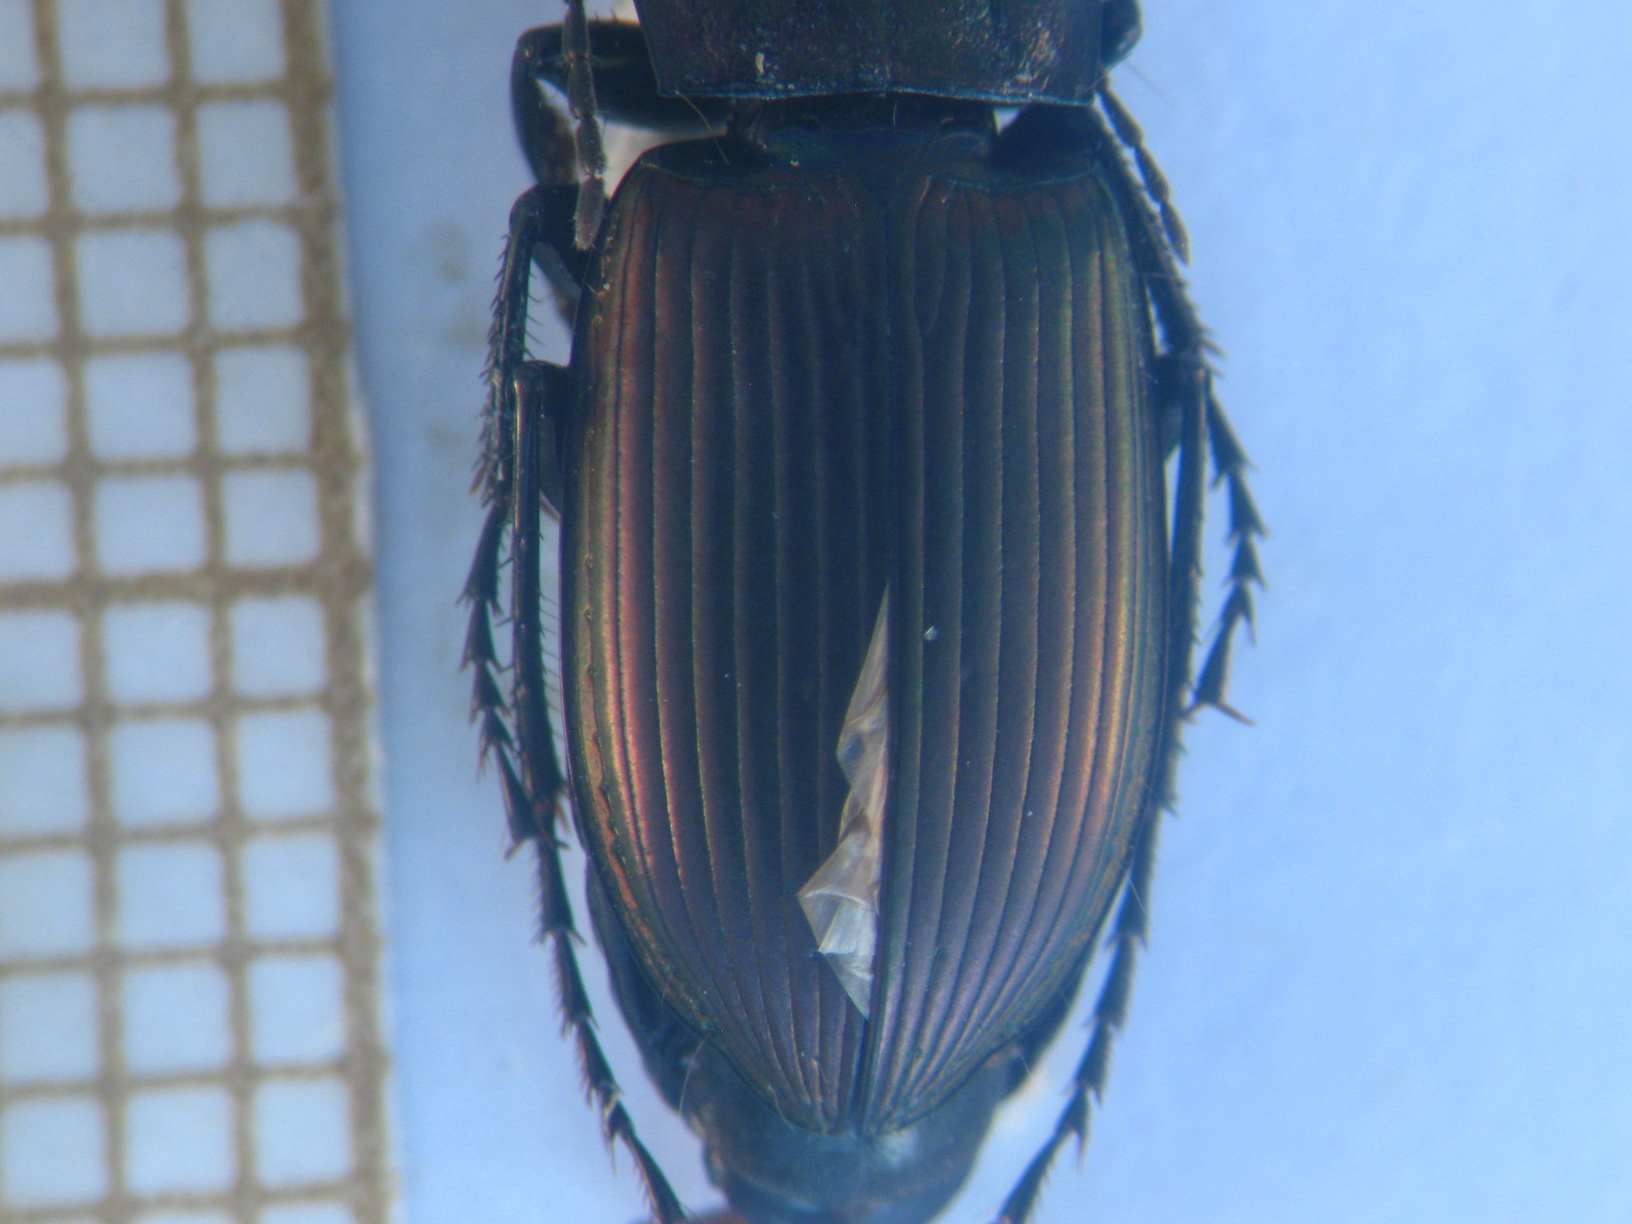
\includegraphics[width=0.4\textwidth]{./images/input1}}~~
\subfloat[The insect overlap the yellow grid]{\label{fig:example_2}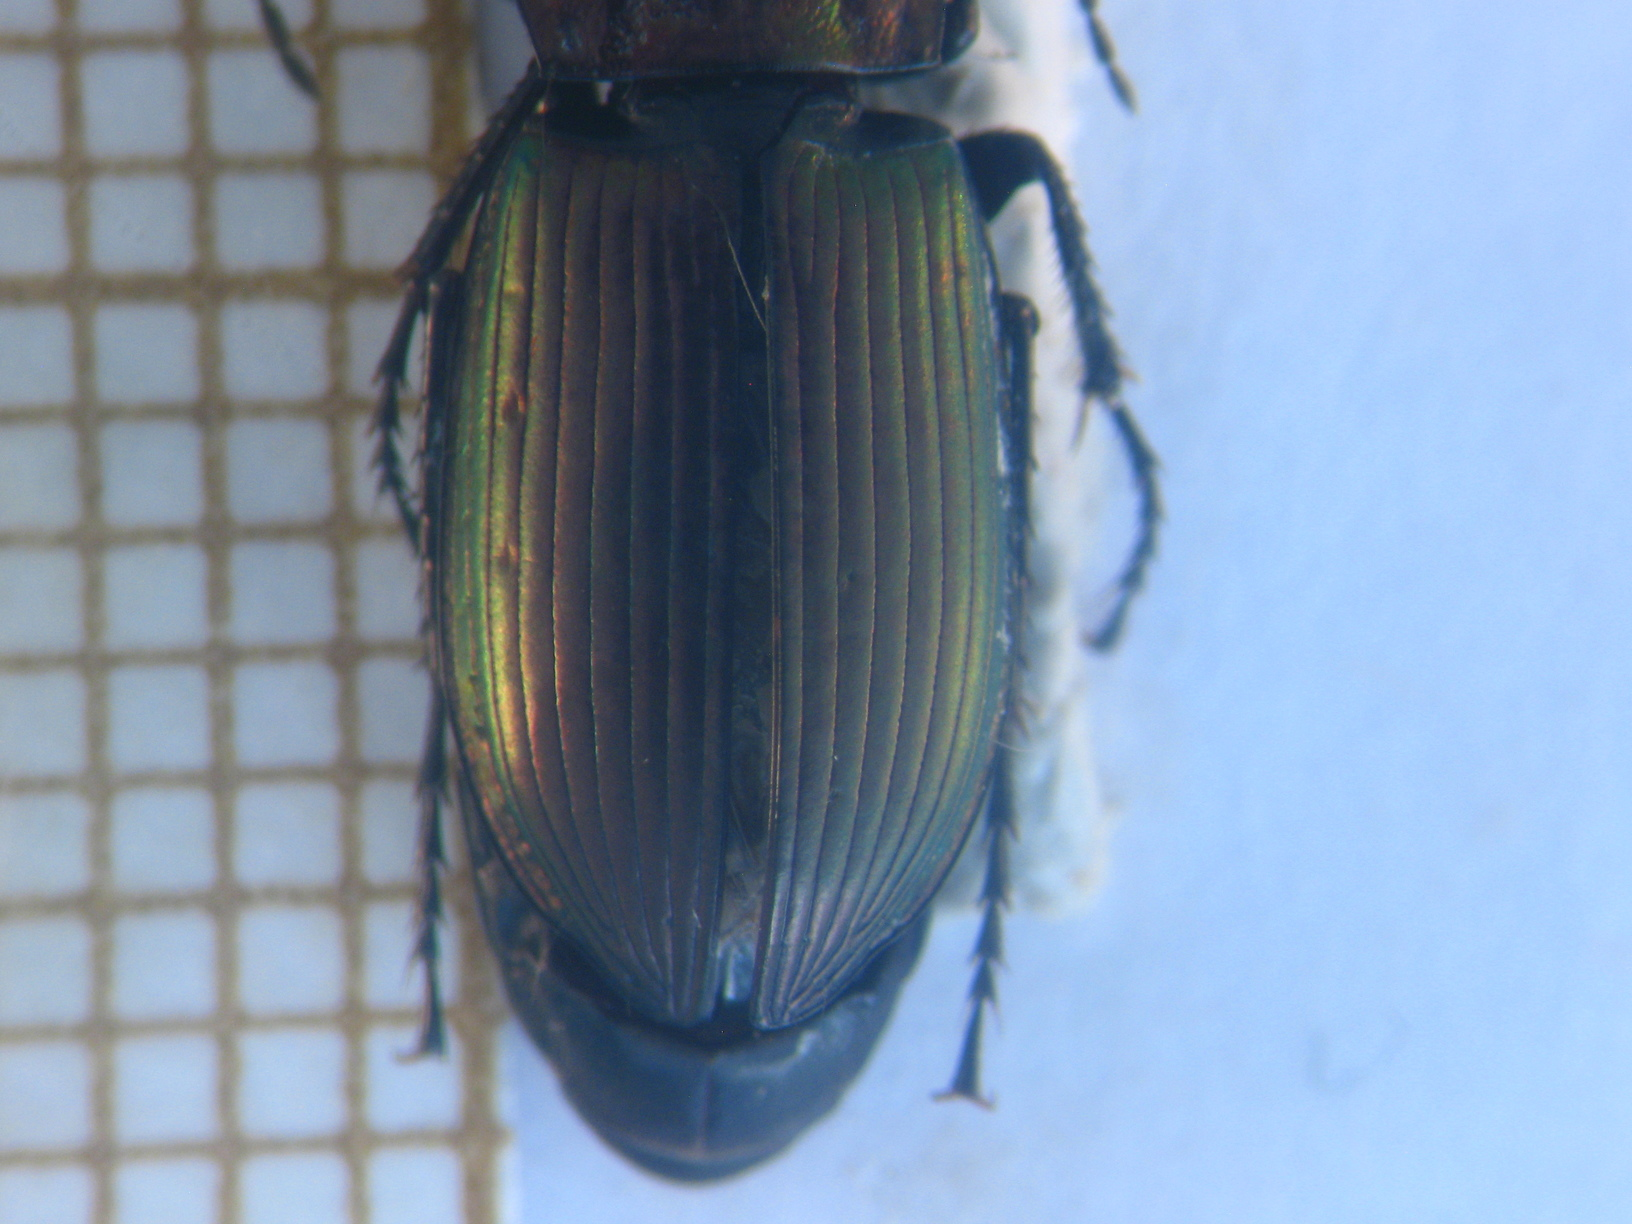
\includegraphics[width=0.4\textwidth]{./images/input2}}
\caption{The input images with yellow grid}
\label{fig:figure_31}
\end{figure}
\section{Analysis}
Each input image contains the two objects: the part of insect and the yellow grid (called grid). Addition, the grid always stay on the left of image, and the insect can either overlap the grid or not. About the color, we can see three main groups color: the background color, the yellow color of grid and the color of insect. The image is presented in BGR model. So, the color at each pixel must be combine among three values (blue, green, red). If we process the image in BGR model, the algorithm may be complex. While, the HSV model just has a channel to present the value of color and each color has a clear range. We can apply this property for detecting and removing the gird.\\
The analysis system is constructed from two main stages: finding the limit points of grid, replacing the yellow point from the begin to the limit point.
\subsection{Finding the limit points}
Browsing all of pixels to checking its color and replacing it if the color of pixel is yellow, we must process on all image. If we do that, it will be waste time. To decreasing the browsing time, in this step we find the limit points. These are the points which located on the right of grid and gird closest.\\
Finding the limit points will solve the above problem. Instance of checking on all pixel, we just check the pixels stay on the left of limit points. As we know, the width of grid usually less than a two-thirds of width of image. So, to reduce the time to finding the limit point, we also check from the begin of image to two-thirds of image. The result of this step is the limit points, these used for limiting the length when we check the pixels on yellow grid.
\subsection{Replacing the grid}
After having the limit points. By processing on all rows of image. At each row, we replace the pixels which have the color value stay in the range of yellow by another value. But the grid is not only created by the yellow point, it contains more the pixel have the value stay in the same range with background. But the brightness of these pixels is less than the background. So, we needs to replace it obtained the good image. In each row, this work repeated until meeting the limit points or a ``special point". It is a point stayed on the insect.
\section{Method}






































